% =====================================================================
%  5.10 PLANIFICACION Y SEGUIMIENTO
%  Rubrica: para "Excelente" hacen falta CUATRO cosas:
%    1. Planificacion presentada
%    2. Seguimiento presentado (datos reales)
%    3. Desviaciones respecto a la planificacion JUSTIFICADAS
%    4. Puntos criticos de la planificacion identificados
%  Presentar solo el Gantt inicial se queda en "Deficiente".
% =====================================================================

\chapter{Planificación y seguimiento}
\label{cap:planificacion}

\section{Planificación inicial}
\label{sec:plan-inicial}

El TFG se planificó para el periodo marzo--agosto de 2026, con una carga de
12~ECTS, equivalente a 300~horas de trabajo del estudiante. Esa cifra fijó
el techo de la estimación inicial. El trabajo se descompuso en cinco fases,
alineadas con la tabla de dedicación de la~\cref{sec:seguimiento}: análisis y
documentación, diseño, implementación, pruebas y redacción de la memoria.

La fase de análisis concentró el estudio de la guía STOPP/START
v3~\cite{omahony2023stopp,sacyl2023stopp}, la delimitación del alcance y la
identificación de lo que debía quedar fuera del producto. El diseño cubrió el
flujo de captura del caso, la organización de la interfaz y el modelo de las
reglas, sin congelar de antemano todos los detalles de presentación. La
implementación absorbió la mayor parte de las 300~horas, por ser la fase en
la que el catálogo, el motor y la interfaz tienen que coexistir en un estado
ejecutable. Las pruebas se planificaron en solapamiento deliberado con la
implementación, de modo que cada incremento pudiera cerrarse con evidencia
de comportamiento y no al final del calendario. La memoria se reservó para
el tramo final, una vez el sistema fuera estable.

El solapamiento entre fases no es un accidente de calendario: el dominio
clínico hace poco realista un diseño en cascada cerrado. Un criterio mal
entendido en análisis reaparece en implementación; un cambio de interfaz
pedido en una ronda de revisión obliga a retocar diseño y código a la vez.
La~\cref{fig:gantt-inicial} muestra el cronograma previsto (barras claras) y
el ejecutado (barras oscuras). El método de trabajo que justifica ese
solapamiento se describe en el~\cref{cap:solucion}; este capítulo se limita
al calendario y a la dedicación.

\begin{figure}[H]
  \centering
  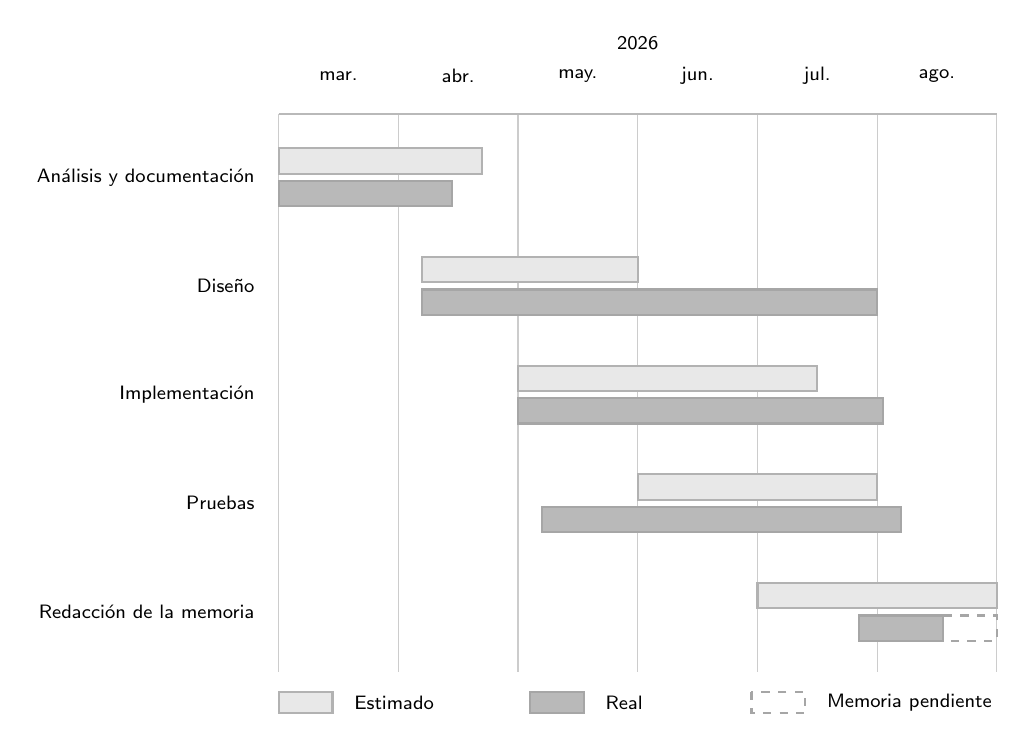
\begin{tikzpicture}[
    x=1.52cm,
    y=-0.46cm,
    font=\footnotesize\sffamily
  ]
    % Rejilla mensual (mar = 0 ... fin de ago = 6)
    \foreach \i in {0,1,2,3,4,5,6} {
      \draw[gray!40] (\i, 1.6) -- (\i, 17.0);
    }
    \draw[gray!55, thick] (0, 1.6) -- (6, 1.6);

    \node[font=\scriptsize\sffamily] at (0.5, 0.55) {mar.};
    \node[font=\scriptsize\sffamily] at (1.5, 0.55) {abr.};
    \node[font=\scriptsize\sffamily] at (2.5, 0.55) {may.};
    \node[font=\scriptsize\sffamily] at (3.5, 0.55) {jun.};
    \node[font=\scriptsize\sffamily] at (4.5, 0.55) {jul.};
    \node[font=\scriptsize\sffamily] at (5.5, 0.55) {ago.};
    \node[font=\scriptsize\sffamily] at (3.0, -0.35) {2026};

    % --- Análisis (est 0.00--1.70; real 0.00--1.45) ---
    \node[anchor=east, align=right, font=\scriptsize\sffamily]
      at (-0.12, 3.35) {Análisis y documentación};
    \fill[gray!18] (0.00, 2.55) rectangle (1.70, 3.25);
    \draw[gray!60, thick] (0.00, 2.55) rectangle (1.70, 3.25);
    \fill[gray!55] (0.00, 3.45) rectangle (1.45, 4.15);
    \draw[gray!70, thick] (0.00, 3.45) rectangle (1.45, 4.15);

    % --- Diseño (est 1.20--3.00; real 1.20--5.00) ---
    \node[anchor=east, font=\scriptsize\sffamily]
      at (-0.12, 6.35) {Diseño};
    \fill[gray!18] (1.20, 5.55) rectangle (3.00, 6.25);
    \draw[gray!60, thick] (1.20, 5.55) rectangle (3.00, 6.25);
    \fill[gray!55] (1.20, 6.45) rectangle (5.00, 7.15);
    \draw[gray!70, thick] (1.20, 6.45) rectangle (5.00, 7.15);

    % --- Implementación (est 2.00--4.50; real 2.00--5.05) ---
    \node[anchor=east, font=\scriptsize\sffamily]
      at (-0.12, 9.35) {Implementación};
    \fill[gray!18] (2.00, 8.55) rectangle (4.50, 9.25);
    \draw[gray!60, thick] (2.00, 8.55) rectangle (4.50, 9.25);
    \fill[gray!55] (2.00, 9.45) rectangle (5.05, 10.15);
    \draw[gray!70, thick] (2.00, 9.45) rectangle (5.05, 10.15);

    % --- Pruebas (est 3.00--5.00; real 2.20--5.20) ---
    \node[anchor=east, font=\scriptsize\sffamily]
      at (-0.12, 12.35) {Pruebas};
    \fill[gray!18] (3.00, 11.55) rectangle (5.00, 12.25);
    \draw[gray!60, thick] (3.00, 11.55) rectangle (5.00, 12.25);
    \fill[gray!55] (2.20, 12.45) rectangle (5.20, 13.15);
    \draw[gray!70, thick] (2.20, 12.45) rectangle (5.20, 13.15);

    % --- Memoria (est 4.00--6.00; real 4.85--5.55, en curso) ---
    \node[anchor=east, font=\scriptsize\sffamily]
      at (-0.12, 15.35) {Redacción de la memoria};
    \fill[gray!18] (4.00, 14.55) rectangle (6.00, 15.25);
    \draw[gray!60, thick] (4.00, 14.55) rectangle (6.00, 15.25);
    \fill[gray!55] (4.85, 15.45) rectangle (5.55, 16.15);
    \draw[gray!70, thick] (4.85, 15.45) rectangle (5.55, 16.15);
    \draw[gray!70, thick, dashed] (5.55, 15.45) rectangle (6.00, 16.15);

    % Leyenda
    \fill[gray!18] (0.00, 17.55) rectangle (0.45, 18.15);
    \draw[gray!60, thick] (0.00, 17.55) rectangle (0.45, 18.15);
    \node[anchor=west, font=\scriptsize\sffamily] at (0.55, 17.85) {Estimado};
    \fill[gray!55] (2.10, 17.55) rectangle (2.55, 18.15);
    \draw[gray!70, thick] (2.10, 17.55) rectangle (2.55, 18.15);
    \node[anchor=west, font=\scriptsize\sffamily] at (2.65, 17.85) {Real};
    \draw[gray!70, thick, dashed] (3.95, 17.55) rectangle (4.40, 18.15);
    \node[anchor=west, font=\scriptsize\sffamily] at (4.50, 17.85)
      {Memoria pendiente};
  \end{tikzpicture}
  \caption{Cronograma del proyecto (marzo--agosto de 2026): barras claras,
  planificación inicial; barras oscuras, ejecución real. La fase de pruebas
  se solapa con la implementación. El tramo discontinuo de la memoria indica
  trabajo aún no cerrado.}
  \label{fig:gantt-inicial}
\end{figure}

\section{Seguimiento: dedicación real}
\label{sec:seguimiento}

Las horas reales de la~\cref{tab:seguimiento} no proceden de un parte de
tiempos diario. Se han reconstruido a partir del histórico de Git ---densidad
y naturaleza de los cambios por mes--- y de la carga de 12~ECTS (300~h) que
fijó la estimación. Marzo corresponde al arranque del repositorio; abril, a
la primera reunión de seguimiento; mayo, al esqueleto de la aplicación;
junio, a la interfaz y a las pruebas de cada incremento; julio, a la
auditoría del catálogo STOPP/START; agosto, a la memoria. La reconstrucción
es una aproximación calibrada para que el plan sume 300~h. La redacción de
la memoria sigue en curso: la cifra real de esa fila es un corte a la fecha
de este capítulo, no el cierre de la fase.

\begin{table}[H]
  \centering
  \begin{tabular}{@{}lrrr@{}}
    \toprule
    \textbf{Fase} & \textbf{Estimado (h)} & \textbf{Real (h)} & \textbf{Desviación} \\
    \midrule
    Análisis y documentación & 40  & 35  & $-5$  \\
    Diseño                   & 45  & 62  & $+17$ \\
    Implementación           & 120 & 148 & $+28$ \\
    Pruebas                  & 50  & 72  & $+22$ \\
    Redacción de la memoria  & 45  & 28  & $-17$ \\
    \midrule
    \textbf{Total}           & \textbf{300} & \textbf{345} & \textbf{$+45$} \\
    \bottomrule
  \end{tabular}
  \caption{Comparación entre la dedicación estimada y la real, en horas, por
  fase. La fila de la memoria está en curso y su valor real es un corte, no
  un cierre.}
  \label{tab:seguimiento}
\end{table}

El total ejecutado (345~h) supera en 45~h la previsión de 300~h. El exceso
se concentra en diseño, implementación y pruebas; análisis y memoria quedan
por debajo, esta última porque aún no ha terminado.

\section{Desviaciones y su justificación}
\label{sec:desviaciones}

Cuatro hechos explican el grueso de las desviaciones positivas. Ninguno de
ellos era un error de cómputo puntual: alteraron el calendario de más de una
fase a la vez.

La primera causa es el diseño de la interfaz. En junio y julio se sucedieron
rondas de revisión con el tutor informático que no estaban dimensionadas en
el Gantt inicial como un bloque de iteración, sino como un diseño
relativamente estable a partir de mayo. Cada ronda exigió reabrir decisiones
de presentación y de flujo ya implementadas, de modo que el diseño se
extendió hasta julio y arrastró retrabajo de implementación. Esa es la
principal explicación de las $+17$~h de diseño. El detalle de las
iteraciones de interfaz corresponde al~\cref{cap:diseno}.

La segunda causa es la auditoría del catálogo STOPP/START, concentrada en
julio. El contraste sistemático con la guía oficial detectó criterios
inventados o redundantes en la sección~B de STOPP y obligó a una revisión
completa de STOPP y de START, no a un arreglo local. El trabajo recayó a la
vez sobre implementación (corregir y completar reglas) y sobre pruebas
(fijar el comportamiento esperado frente al texto de la guía). Es la
contribución mayor a las $+28$~h de implementación y una parte de las
$+22$~h de pruebas. Los fallos concretos hallados en el catálogo se
recogen en el~\cref{cap:pruebas}; aquí basta constatar que una auditoría de
ese alcance no estaba prevista como un mes entero de calendario.

La tercera causa es una funcionalidad de historial de casos que llegó a
implementarse y después se eliminó. Consumió diseño, código y pruebas de un
recorrido que no forma parte del flujo fusionado. El coste no se recupera
al borrar la feature: el tiempo ya se había empleado. Forma parte del
exceso de implementación y, en menor medida, del de pruebas.

La cuarta causa es el mantenimiento de una batería de pruebas junto con
guardas sobre el catálogo a lo largo de toda la implementación, no solo al
final. Esa disciplina ---descrita en el~\cref{cap:solucion}--- alarga cada
incremento, explica el resto de las $+22$~h de pruebas y adelanta el inicio
real de esa fase a mayo (\cref{fig:gantt-inicial}). El inventario pertenece
al~\cref{cap:pruebas}.

Las desviaciones negativas tienen justificación simétrica. El análisis
cerró cinco horas por debajo porque el dominio venía acotado por una guía
publicada. La memoria lleva diecisiete horas menos porque julio se destinó
a la auditoría y a las rondas de interfaz, y la redacción se desplazó a
agosto, donde todavía continúa.

\section{Puntos críticos identificados}
\label{sec:puntos-criticos}

Tres puntos condicionaban al resto del calendario. Se identificaron en el
análisis y se confirmaron en la ejecución.

El primero es la formalización de los 190 criterios de la guía como reglas
evaluables. Hasta que un criterio no está expresado de forma unívoca, no hay
aviso que mostrar ni prueba significativa. Un error aquí bloquea el catálogo
y degrada cualquier fecha posterior. El volumen ---133 STOPP y 57
START~\cite{omahony2023stopp}--- impedía tratarla como relleno final: tenía
que avanzar sistema a sistema. La auditoría de julio lo confirmó: un
conjunto pequeño de criterios mal codificados en una sección obligó a
revisar el catálogo entero.

El segundo es la decisión temprana de un motor declarativo: las reglas viven
aparte del mecanismo que las aplica. Esa elección fija el formato del
catálogo y el orden de la implementación. Codificar cada criterio como rama
de programa habría cambiado el calendario de corrección y habría reabierto
código ante cada actualización de la guía. El resto de fases asumía que el
catálogo podía crecer sin reescribir la aplicación. El~\cref{cap:arquitectura}
desarrolla esa decisión; aquí importa que era un hito de camino crítico.

El tercero es el riesgo de falso negativo clínico: un criterio que debería
activarse y no lo hace. El profesional no ve el aviso, de modo que el fallo
es más grave que un aviso espurio. No es una barra del Gantt, pero
condiciona el cierre: no se podía terminar un sistema de criterios sin
contrastarlo con la guía, ni comprimir las pruebas para recuperar retraso de
interfaz. En julio se priorizó la auditoría frente a adelantar la memoria.
El~\cref{cap:solucion} justifica esa prioridad; el~\cref{cap:pruebas}
documenta cómo se comprobó.
